\documentclass[11pt]{article}

\usepackage[utf8]{inputenc}
\usepackage[english, ukrainian]{babel}
\usepackage{amssymb,latexsym,amsmath,amscd,amsthm, mathtools}

\usepackage{biblatex}
\addbibresource{stereo_vision.bib}

\usepackage{graphicx}
\graphicspath{{./assets/}}
\usepackage{caption}
\usepackage{subcaption}
\usepackage{setspace}
\usepackage{listings}

\newtheorem{theorem}{Теорема}
\newtheorem*{theorem*}{Теорема}
\newtheorem{proposition}{Твердження}
\newtheorem*{example*}{Приклад}
\theoremstyle{definition}
\newtheorem*{exercise}{Задача}
\newtheorem{definition}{Означення}[section]

\newcommand{\sToInf}[1]{\sum\limits_{#1=1}^{\infty}}
\newcommand{\abs}[1]{\left\lvert #1 \right\rvert}
\newcommand{\norm}[1]{\left\lVert#1\right\rVert}

\begin{document}

\begin{titlepage}
	{\setstretch{1.5}
		\centering \mbox{КИЇВСЬКИЙ НАЦІОНАЛЬНИЙ УНІВЕРСИТЕТ ІМЕНІ ТАРАСА ШЕВЧЕНКА}
		
		\centering МЕХАНІКО-МАТЕМАТИЧНИЙ ФАКУЛЬТЕТ
		
		\centering КАФЕДРА АЛГЕБРИ І КОМП’ЮТЕРНОЇ МАТЕМАТИКИ
		
	}
	
	\vspace{30pt}

	\noindent
	Освітній ступінь: магістр \\ \\
	за спеціальністю 111 - математика \\
	за освітніми програмами - математика
	
	\vspace{30pt}
	
	{
		\noindent \centering кваліфікаційна робота на ступінь магістра математики
		
		\noindent \centering на тему “Застосування машинного навчання у задачі знаходження відповідностей для стерео пари”
		
	}
	
	\vspace{30pt}
	
	\begin{flushright}
		студента 2 курсу магістратури \\
		Швеця Максима Сергійовича
	\end{flushright}

	\vspace{30pt}

	\noindent
	Допущений до захисту в ЕК \\
	Протокол №11 засідання кафедри \\
	алгебри і комп’ютерної математики \\
	від 21 квітня 2020 року
	
	\vspace{30pt}
	
	\begin{flushright}
		Науковий керівник \\
		Доктор фізико-математичний наук \\
		Лавренюк Я. В.
	\end{flushright}

	\vspace*{\fill}
	\centering Киів-2020
\end{titlepage}

\newpage

\tableofcontents

\newpage

\section{Огляд}
В цій роботі розглянемо задачу стереобачення та метод її розв’зання за допомогою машинного навчання запропонований в статті “Efficient Deep Learning for Stereo Matching” \cite{deepLearningForStereo}. Модифікуємо цей метод та перевіримо його еффективність на датасеті KITTI.

\section{Стереобачення}
Задача стереобачення полягає в знаходженні інформації про тривимірні об'єкти використовуючи їх зображення. Зазвичай розглядають два зображення отримані з двох камер розташованих на одній горизонтальній осі, саме з такими данними працює алгоритм описаний в цій роботі.

Маючи два зображення однїєї сцени можна зрозуміти наскільки далеко розташовані від камери зображені об'єкти спостерігаючи за зміною їх положення на зображеннях. Чим сильніше змінюється положення об'єкта між зображеннями, тим ближчий він до камери. Приклад цього можна побачити на рис. \ref{fig:tsukuba_stereopair} взятому із датасету MIddlebury \cite{middlebury2001dataset}.

\begin{figure}[h]
	\begin{subfigure}{.5\textwidth}
		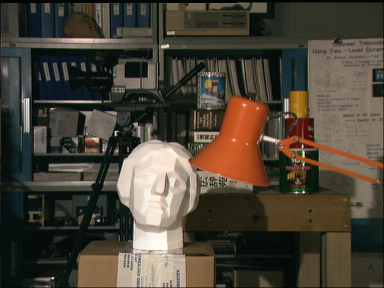
\includegraphics[width=0.9\linewidth]{disparity_example_left}
		\centering
	\end{subfigure}
	\begin{subfigure}{.5\textwidth}
		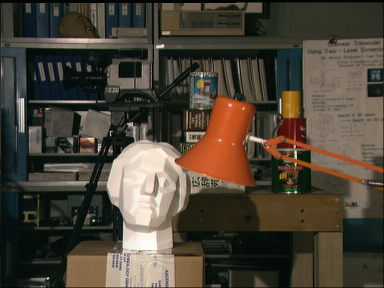
\includegraphics[width=0.9\linewidth]{disparity_example_right}
		\centering
	\end{subfigure}
	\caption{Настільна лампа розташована ближче до камери і тому ссувається сильніше ніж, наприклад, голова чи стіл}
	\centering
	\label{fig:tsukuba_stereopair}
\end{figure}

Якщо для деякої точки сцени відомі відповідні їй точки на зображеннях, то ми можемо розрахувати глибину цієї точки за формулою (рис. \ref{fig:tirangulation_showcase}). 
\[ h = \frac{fb}{d} \]
де $f$ - це фокусна відстань, $b$ - відстань між камерами, $d$ - різниця між кординатами точок зображеннь. Також, можна розрахувати відстань від оптичної вісі камери за формулою
\[ r = \frac{bx_r}{d} \]
де $x_r$ - відстань точки від центра зображення

\begin{figure}[h]
	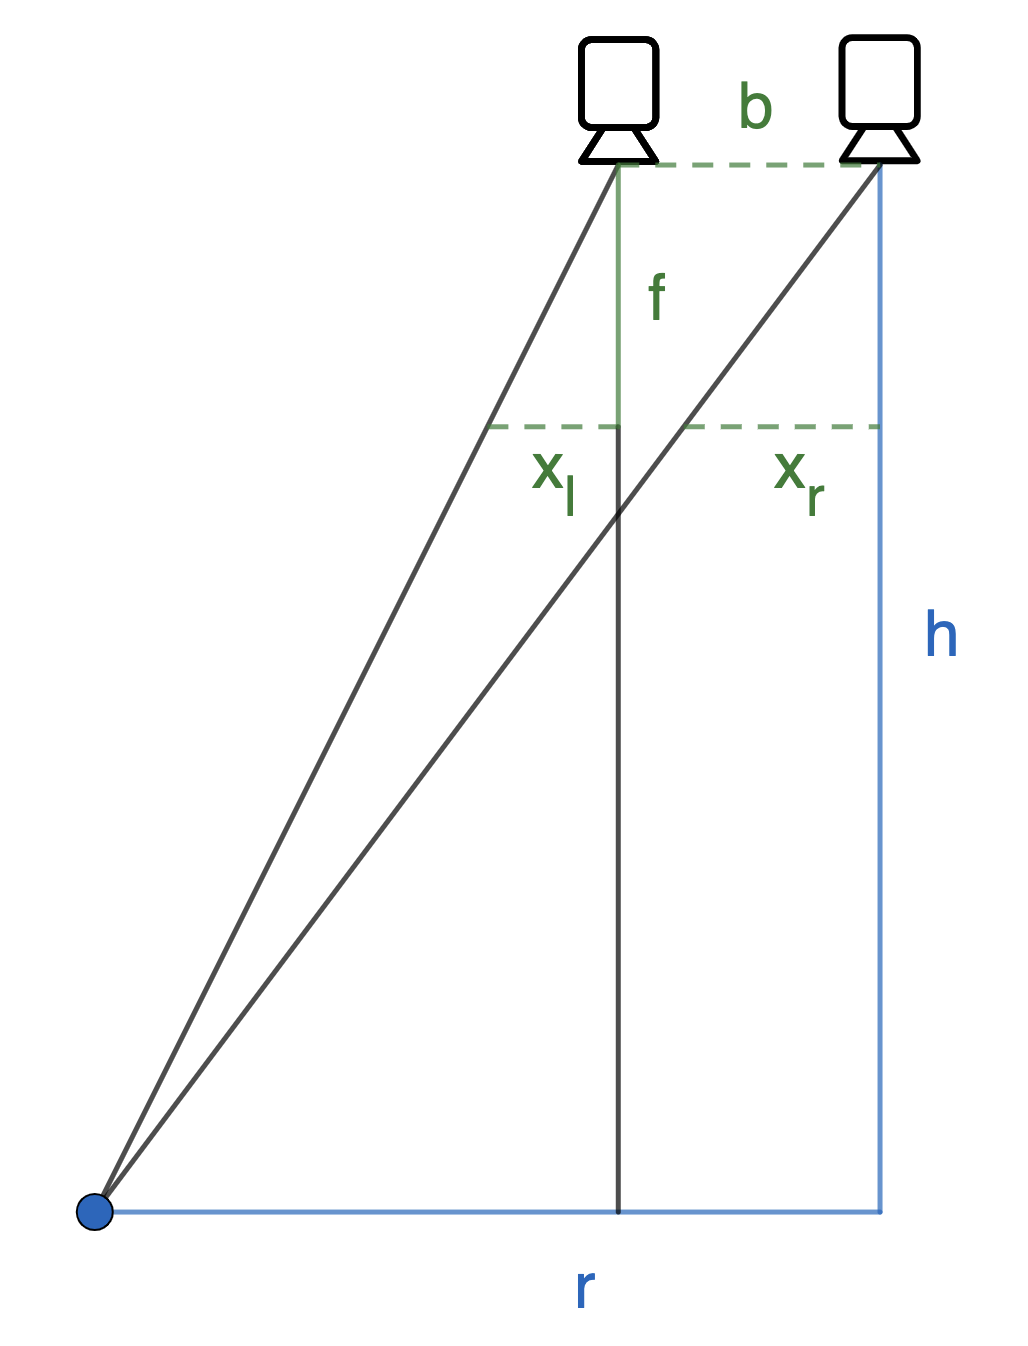
\includegraphics[width=0.7\linewidth]{triangulation_with_cameras}
	\centering
	\caption{Відомі нам значення (відстань між камерами $b$, фокусна відстань $f$, координати точок на зображеннях $x_l, x_r$ позначено синім. Значення які можемо знайти (глибина зображення - $h$, відстань від вісі камери - $r$) позначено зеленим)}
	\label{fig:tirangulation_showcase}
\end{figure}

Отже, маючи алгоритм який співставляє точкам одного зображення відповідні їм точки іншого зображення ми можемо знаходити відстані до точок сцени. Зручний спосіб представити ці відстані - чорно-біле зображення в якому кожен піксель тим світліший чим більше значення $d$ його зсуву на іншому зображенні. Це зображення називають \textbf{мапою зсувів} (англ. disparity map). За попередньої форму видно що зсув обернено-пропорційний глибині, тому об'єкти на такому зображені будуть тим світліші чим ближче вони до камери. Мапу зсувів для стереопари зображенної на рис. \ref{fig:tsukuba_stereopair} можна побачити на рис. \ref{fig:tsukuba_disparity}. 

\begin{figure}[h]
	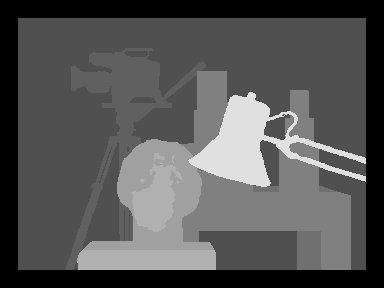
\includegraphics[width=0.5\linewidth]{disparity_map_example}
	\centering
	\caption{Лампа знаходиться ближче до камери тому зсув пікселів на яких зображена лампа вищий, а отже на малюнку вони світліші.}
	\label{fig:tsukuba_disparity}
\end{figure}

Розгянутий алгоритм приймає два зображення і обчислює мапу зсувів.

\subsection{Виправлення зображеннь}
Знаходити відповідні пікселі легше за все коли камери зміщені лише горизонтально і направлені однаково. При такому налаштуванні пікселі будуть зсуватись між зображеннями лише по горизонталі, а отже ми можемо шукати відповідні пікселі лише в одному вимірі.

\begin{figure}[h]
	\begin{subfigure}{.5\textwidth}
		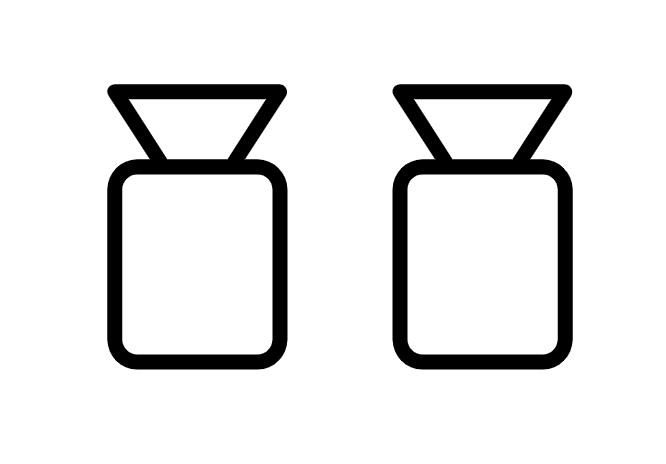
\includegraphics[width=0.6\linewidth]{cameras_conveniently_placed}
		\centering
		\caption{Зручне розташування}
	\end{subfigure}
	\begin{subfigure}{.5\textwidth}
		
\includegraphics[width=0.9\linewidth]{cameras_inconveniently_placed}
		\centering
		\caption{Незручне розташування}
	\end{subfigure}
	\centering
	\label{fig:camera_positions}
\end{figure}

У випадках коли цих ідеальних умов неможливо досягти, до зображень можна застосувати процедуру виправлення (англ. rectification), яка полягає в проектуванні зображеннь на одну площину. Результат застосування такої процедури можна побачити на рис. \ref{fig:rectification_example}.

\begin{figure}[h]
	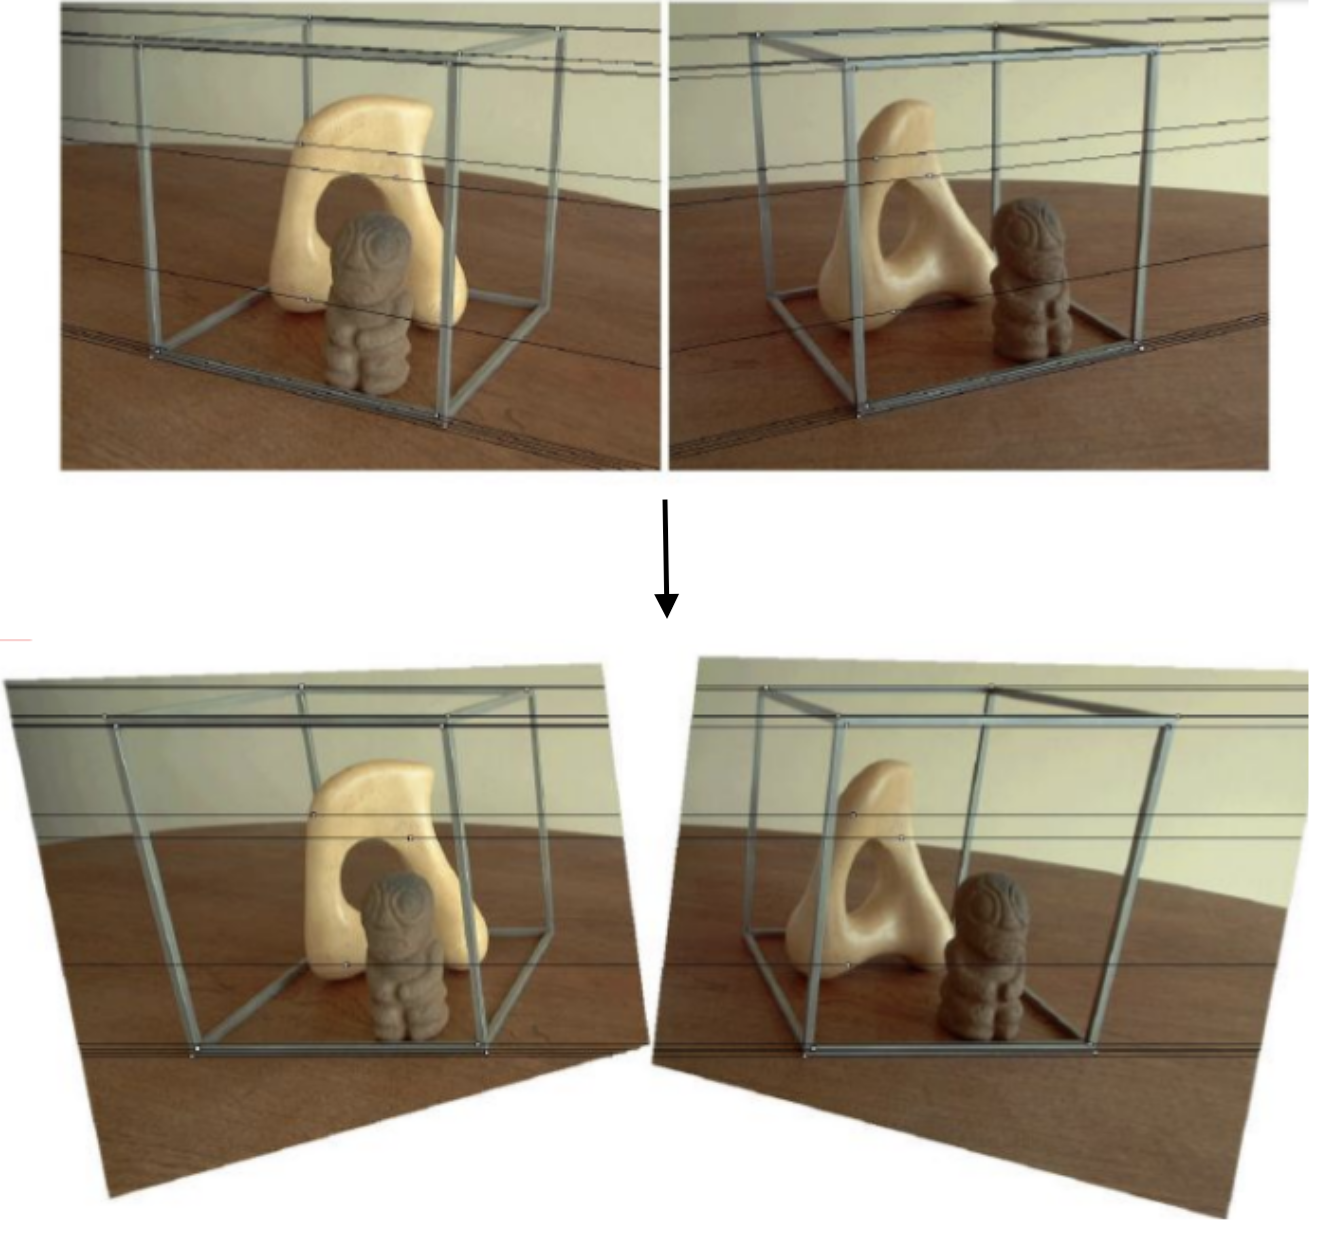
\includegraphics[width=0.7\linewidth]{rectification_example}
	\centering
	\caption{Приклад виправлення зображень}
	\label{fig:rectification_example}
\end{figure}

\subsection{Релевантність}
Задача стереобачення важлива в таких областях як роботехніка, об'ємна відбудова (англ. 3D scene reconstruction), безпілотне вождіння та побудова доповненої реальності.

\section{Алгоритм}
\subsection{Базовий алгоритм}
Типовий алгоритм розв'язання задачі стереобачення починає з підрахунку cost-функції для кожного можливого значення зсуву. Ми хочемо щоб cost-функція мала низьке значення для зсувів близьких до реального і велике значення для зсувів далеких від реального. 
\begin{example*}
	Cost-функцію можна визначити як суму абсолютних різниць.
	\[ Cost(x_0, y_0, d) = \sum_{(x, y) \in W(x_0,y_0)} \left| I^L(x, y) - I^R(x - d, y) \right| \]
	Тут $I^L(x,y), I^R(x,y)$ інтенсивності пікселів з координатами $(x,y)$ на лівому та правому малюнку відповідно, а $W(x,y)$ окіл пікселя $(x,y)$. Отже, ця функція порівнює інтенсивності пікселів в околах $(x_0, y_0)$ і $(x_0 - d, y_0)$. Якщо ці пікселі відповідають одній і тій самій 3D точці, то інтенсивності в їх околах скоріш за все будуть майже однаковими і значення функціі буде відносно низьким.
\end{example*}

Простий вибір тих зсувів для яких значення cost-функції найбільш низьке зазвичай приводить до поганих результатів (як ми побачимо пізніше), тому результати обчислення cost-функції додатково оброблюются. Методи обробки не залежать від способу підрахунку cost-функції, для розглянутого алгоритму використані добре відомимі методи які буде наведено пізніше.

З появою великих датасетів таких як KITTI и Middleburry, в яких для різних стереопар доступна справжня карта зсувів (отримана за допомогою LIDAR чи структурованого світла), стало можливим застосування машинного навчання для того щоб обчислювати cost-функцію. Ми використовуємо датасет KITTI щоб натренувати нейронну мережу що буде розраховувати cost-функцію.

\subsection{Структура нейронної мережі}
На рис. \ref{fig:nn_structure} зображенно структуру нейронної мережі. Далі наведемо визначення використаних блоків:
\begin{itemize}
	\item \textit{ConvBNReLu(in, out, w, h)} - поєднання декількох інших блоків: 
	
	\textit{Convolution(in, out, w, h)} $\to$ \textit{BatchNormalization(out, $0.001$)} $\to$ \textit{ReLU}
	
	\item \textit{Convolution(in, out, w, h)} - приймає тензор з вимірами $in \times x \times y$, виконує $out$ згорток з $in \times w \times h$ тензором і повертає результат у вигляді $out \times x^* \times y^*$ тензора, де 
	\[ x^* = x - w + 1, \  y^* = y - h + 1 \]
	
	\item \textit{BatchNormalization(in, esp)} - приймає тензор з вимірами $in \times x \times y$ і повертає тензор з такими самими вимірами. Детальніше про цей шар можна почитати в статі \cite{ioffe2015batch}.
	
	\item \textit{ReLU} - застосовує $max(0, x)$ до кожного елемента тензора
	
	\item \textit{DotProduct} - підраховує скалярний добуток тензорів
	
	\item \textit{LogSoftMax} - приймає вектор $(x_i)_{i=1}^n$ і розраховує 
	\[ \left( log\left( \frac{e^{x_i}}{S} \right) \right)_{i=1}^n \]
	де $S = \sum_{i=1}^n e^{x_i}$
\end{itemize}

Позначення $5*$\textit{ConvBNReLU} значить блок \textit{ConvBNReLU} застосований 5 разів.
	
\begin{figure}[h]
	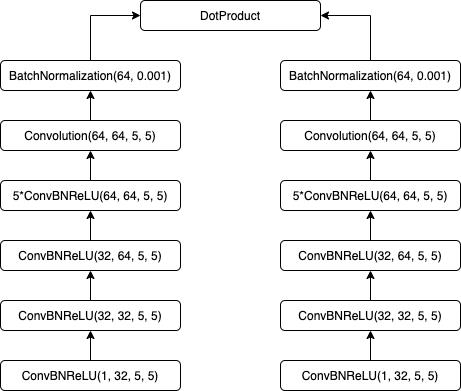
\includegraphics[width=\linewidth]{nn_structure_prod}
	\centering
	\caption{Структура нейронної мережі}
	\label{fig:nn_structure}
\end{figure}

\subsection{Застосування нейронної мережі}
Щоб застосувати нейронну мережу до зображень зі стереопари, зображення подаються у вигляді тензорів з вимірами $c \times w \times h$, де $c=1$ якщо зображення чорно-біле (один канал кольору) і $с=3$ якщо зображення кольорове (три канали кольору). Будемо позначати ці тензори $P^L_{c, w, h}$ і $P^R_{c, w, h}$ для правого і лівого зображення відповідно. Також, оскільки кожен згорточний шар нейронної мережі зменшує ширину та висоту тензора, до зображень додається прослойка так щоб на виході ширина та висота тензора була рівна ширині та висоті зображення. Отже, в нашому випадку в нейронну мережу передаються тензори $P^L_{c, w+36, h+36}, P^R_{c, w+36, h+36}$, бо кожен з $9$ згорткових шарів нейронної мережі зменшує виміри на $4$, і на виході отримуються тензори
\[ O^L_{64, w, h} := (o^l_{i,j,k})_{i=1,j=1,k=1}^{64,w,h} \]
\[ O^R_{64, w, h} := (o^r_{i,j,k})_{i=1,j=1,k=1}^{64,w,h} \]

Cost-функція розраховується за формулою:
\[ Cost(x, y, d) = - \langle O^L(x, y), O^R(x - d, y) \rangle \]
де $O^L(x, y) = (o^l_{i,x,y})_{i=1}^{64}$, $O^R(x, y) = (o^r_{i,x,y})_{i=1}^{64}$, а $\langle \cdot, \cdot \rangle$ позначає скалярний добуток.

\textbf{Як інтерпретувати цю cost-функцію?} Кожна гілка нейронної мережі знаходить деякі характерні риси в частині малюнка навколо пікселя. Які саме риси буде шукати мережа визначається під час тренування, оскільки ми використовуємо однакові параметри для обох гілок, вони будуть шукати однакові риси. Кожне з 64 чисел на позиції $(x, y)$ показує наскільки властива одна з 64 рис частині малюнка навколо $(x,y)$. Отже, кожна $i$-та компонента вектора $O^L(x,y)$ показує наскільки властива цій частині зображення $i$-та риса, так само для правого зображення і вектора $O^R(x,y)$. Чим більш схожі риси описані в цих векторах, тим більшим буде скалярний добуток і тим менше буде cost-функція

Якщо для кожного пікселя $(x,y)$ просто взяти те значення $d$ для якого значення cost-функції найменше, отримаємо досить поганий результат (див. рис. \ref{fig:bad_approach_example}), тому результати нейронної мережі додадтково оброблюються. Як саме буде описано далі.

 \begin{figure}[h]
 	\begin{subfigure}{\textwidth}
 		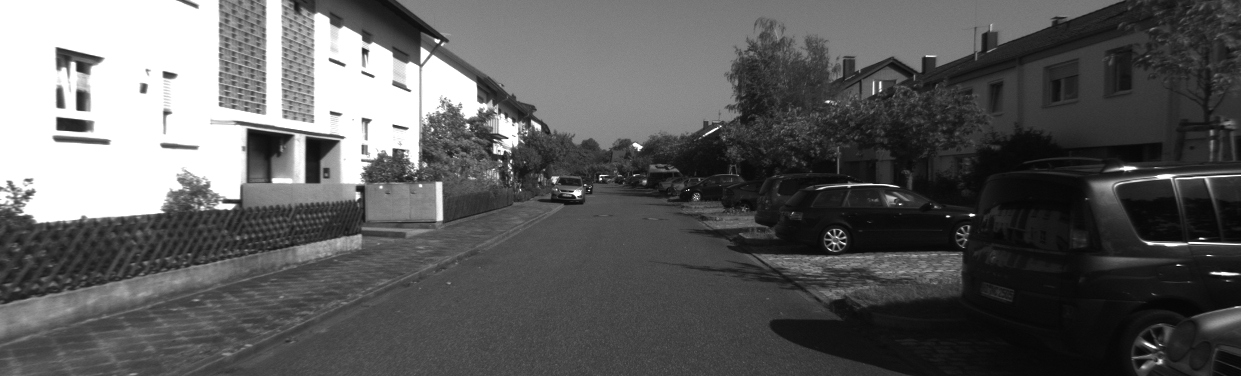
\includegraphics[width=\linewidth]{kitti_example_left}
 		\centering
 	\end{subfigure}
 	\begin{subfigure}{\textwidth}
 		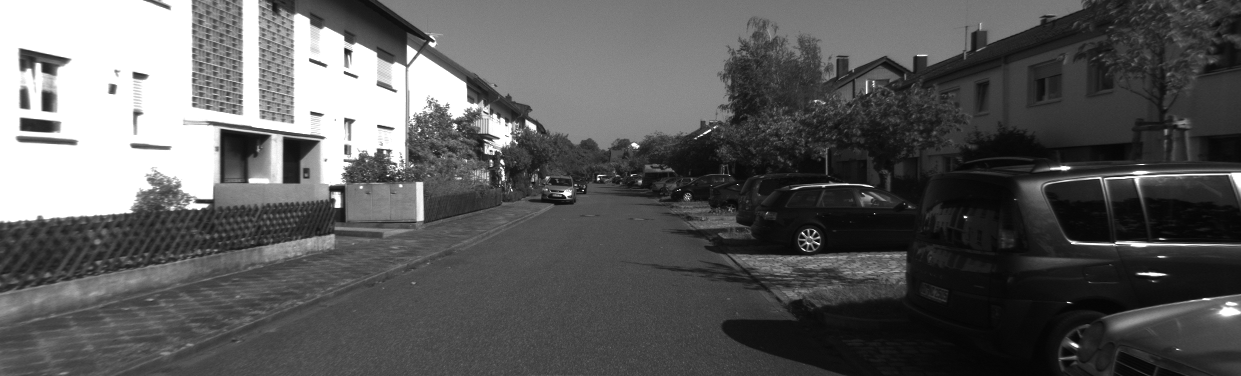
\includegraphics[width=\linewidth]{kitti_example_right}
 		\centering
 	\end{subfigure}
	\begin{subfigure}{\textwidth}
		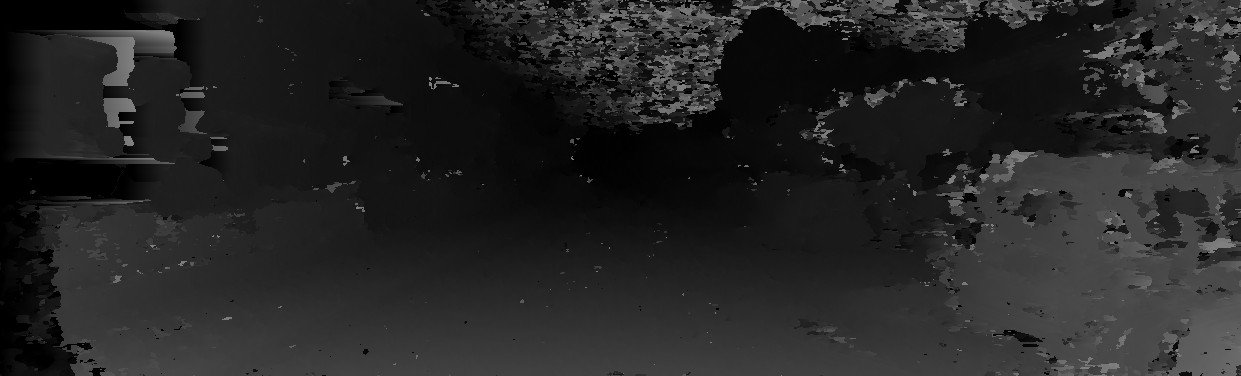
\includegraphics[width=\linewidth]{no_smoothing_result}
		\centering
	\end{subfigure}
 	\centering
 	\caption{Приклад результатів без застосування згладжування}
 	\label{fig:bad_approach_example}
 \end{figure}

\newpage

\section{Тренування}
Чи буде мережа добре обчислювати cost-функцію залежить від значень параметрів в її згорткових блоках. Параметрами згорткового блока є числа в тензорах з якими він виконує згортку.
\begin{example*}
	Блок \textit{Convolution}$(32, 64, 5, 5)$ виконує $64$ згортки з різними тензорами вимірів $32 \times 5 \times 5$. Результатом кожної згортки є матриці $x^* \times y^*$ з яких формується результат. Числа в кожному з тензорів є параметрами цього блоку. Отже, блок \textit{Convolution}$(32, 64, 5, 5)$ має $64 * 32 * 5 * 5 = 51200$ параметрів. Вся нейронна мережа містить $693536$ параметрів
\end{example*} 

Очевидно, кількість параметрів занадто велика для того щоб обрати їх значення вручну. 
Тому значення параметрів обираються програматично, спираючись на набір стереопар для яких відомі мапи зсувів. Узагальнене описання алгоритму тренування таке:
\begin{enumerate}
	\item Ініціалізуемо параметри випадковими значеннями
	\item Підраховуємо функцію витрат для поточних значень параметрів. 
	\item Підраховуємо градієнт функції витрат для поточних параметрів
	\item Змінюємо параметри у напрямі протилежному напряму градієнту
	\item Повторюємо кроки 2-4 доки не знайдемо мінімум функції витрат
\end{enumerate}

\textbf{Функція витрат} оцінює наскільки сильно результати роботи мережі відрізнются від справжніх результатів (які нам наперед відомі). Чим більша різниця між отриманими та справжніми результатами, тим більше значення функції витрат для параметрів. Її значення зазвичай підраховується шляхом застосування нейронної мережі і порівняння її результатів з наперед відомими правильними результатами. Для того щоб підрахувати градієнт функції витрат зазвичай використовують алгоритм backpropagation. Далі опишемо процес тренування більш детально.

\subsection{Побудова датасету для тренування}
Введемо деякі позначення. Будемо позначати $W^L_{w,h}(x,y)$ вікно розміру $w \times h$ з центром в пікселі $(x,y)$. $W^R_{w,h}(x,y)$ буде означати те саме для правого зображення.

Для того щоб побудувати датасет на якому тренується нейронна мережа використано данні з датасету KITTI, який містить приблизно 200 стереопар для яких відомі значення зсувів. З кожної стереопари, для тих пікселів лівого зображення $(x, y)$ для яких відоме значення зсуву $d$, jобирається пара $W^L_{37,37}(x,y)$, $W^R_{37 + 2D,h}(x - d,y)$, де $D$ - максимальне абсолютне значення зсуву. Всі такі пари і складають остаточний датасет.

\subsection{Підхід до тренування}
При тренуванні задача стереобачення розглядається як задача класифікаціЇ. Тобто, структура нейронної мережї дещо змінюється так, щоб на виході вона давала вектор довжини $D$, в якому $i$-а компонента містить ймовірність того що значення зсуву рівне $i$. Далі детальніше опишемо ці зміни.
  
На відміну від нейронної мережі яка використовується на реальних данних, під час тренування результати гілок об'єднуються матричним добутком. Оскільки при обробці $W^L_{37,37}(x,y)$ лівою гілкою отримуємо вектор з $64$ значень, а при обробці $W^R_{37 + 2D,h}(x - d,y)$  отримуємо матрицю $D \times 64$, то матричний добуток дає вектор з $D$ значень. До цього вектора застосовується $LogSoftMax$ функція (визначення якої наведено вище), що й обчислює шукані ймовірності.

Оскільки єдина части нейронної мережі що має параметри це її гілки, то така зміна структури не впливає на роботу остаточної нейронної мережі.

\subsection{Функція витрат}
В якості функції витрат використовується
\[ L(x, d_t) = -x_{d_t} \]
де, $x$ - вектор ймовірностей розрахований нейронною мережею, $d_t$ - справжнє значення зсуву.

Тобто, щоб порахувати функцію витрат для заданого набору параметрів, нейронна мережа спочатку застосовується до стереопари, а потім береться ймовірність порахована для справжнього значення зсуву зі знаком мінус.

\section{Згладжування}
Як ми вже побачили, однієї лише нейронної мережі недостатньо для того щоб отримати якісну мапу зсувів, тому результати нейронної мережі проходять пост-процессинг. Для пост-процессингу використовуємо методи детально описані в статі \cite{zbontar2016stereo}. Тут надамо лише їх поверхневий опис.

\subsection{Cost агрегація}
Для кожного пікселя рахує середнє значеннь cost-функції в околі розміру $5 \times 5$. Зауважимо, що середнє підраховується окремо для кожного значення зсуву.

\subsection{Перехрестна cost агрегація}
Цей метод спочатку будує окіл для кожного пікселя уникаючи того щоб околи переходили через края об'єктів на зображенні. Щоб досягти цього,  побудова околу починається з одного пікселя, до якого додаються сусідні пікселі доки їх інтенсивність і відстань до початкового пікселя знаходится в заданих межах.

Маючи околи, метод рахує середнє значень cost-функцій в них. Цей крок повторюється чотири рази

\subsection{Semiglobal matching}
Визначає енергетичний функціонал який залежить від мапи зсувів і штрафує мапи з великими значеннями cost-функцій та мапи в яких значення зсувів для сусідніх пікселів сильно відрізняються. Цей функціонал мінімізується у декількох напрямках.

\subsection{Поєднання методів}
Наведені вище методи поєднуються наступним чином:
\begin{itemize}
	\item Використовується cost агрегація
	\item Використосується перехрестна cost агрегація
	\item Використовується semiglobal matching
	\item Використосується перехрестна cost агрегація
\end{itemize}

Після наведенних вище кроків до отриманні значення додатково оброблюються методами описанними в \cite{zbontar2016stereo}

\subsection{Результати згладжування}
На рис. \ref{fig:smoothing_result} можна побачити результати застосування сгладжування до прикладу з рис. \ref{fig:bad_approach_example}
\begin{figure}[h]
	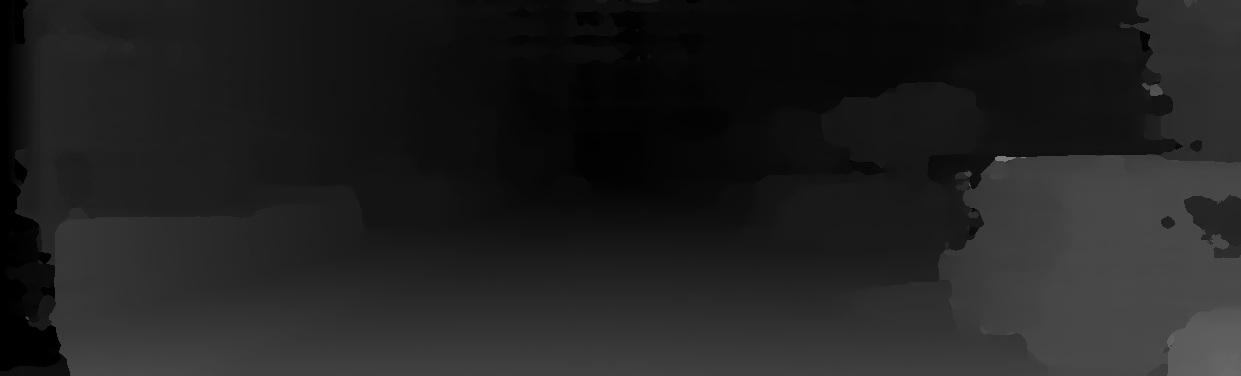
\includegraphics[width=\linewidth]{smoothing_result}
	\centering
	\caption{Результати після застосування сгладжування}
	\label{fig:smoothing_result}
\end{figure}

\newpage

\printbibliography 

\newpage

\section*{Додаток 1}
Процедура вибору данних для тренувального датасету
\lstinputlisting[language=Octave]{assets/extract_patches.m}

\end{document}